\chapter{Caso de uso}
\label{caso_de_uso}

\section{Justificación del algoritmo}
\label{justificacion}

\comment{??}

\section{Problema}
\label{problema}

El programa realizado se basa en una aplicación típica de robots rastreadores de competición. En estas competiciones, los robots pasan por diferentes pruebas, como encontrar la salida de un laberinto o cruzar un escenario con obtáculos. En la figura \ref{fig:competi1}, puede observarse cómo estos obstáculos generalmente no tienen texturas y utilizan formas muy básicas. Con esto se intenta abstraer al robot de perturbaciones físicas y visuales, presentando un entorno modular y simple.

\begin{figure}[h]
		\centering
        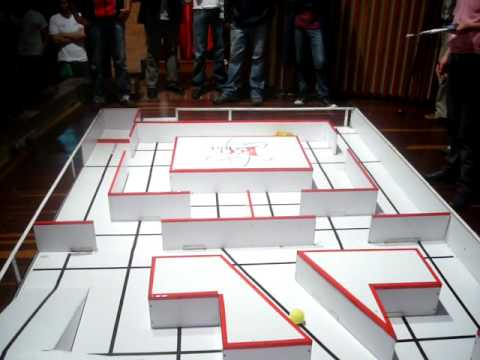
\includegraphics[width=0.5\textwidth]{images/competi1.jpg}
        \caption{Escenario de competición robótica}
        \label{fig:competi1}
\end{figure}  

El uso de obstáculos modulares permite simular una gran cantidad de casos problemáticos, siendo muy fácil reconfigurar su posición y unir obstáculos para crear obstáculos más complejos.

En el programa desarrollado, el robot pasará un total de tres pruebas diferentes en las que se combinarán distintos obstáculos frecuentes en las competiciones de robots rastreadores. Además, se tendrá en cuenta el tiempo usado en recorrer el escenario, por lo que se intentará minimizar.



\section{Ámbito de uso}
\label{ambito}

\comment{?? limitaciones??}